\subsection{Polar Basis Vectors}
\begin{definition}[Polar Orthonormal Basis]
	{\bf Unit Vectors} $$\underline{e_r} \ \ \  \text{and} \ \ \ \underline{e_{\theta}}$$
	form the {\bf orthonormal basis} for  the {\bf The Polar Co-Ordinate System}.
\end{definition}

Furthermore, the unit vectors $\underline{e_r}$ and $\underline{e_{\theta}}$ can be represented using {\bf cartesian basis vectors} $\underline{i}$ and $\underline{j}$

\begin{mycenter}
	\tikzset{every picture/.style={line width=0.75pt}} %set default line width to 0.75pt        

	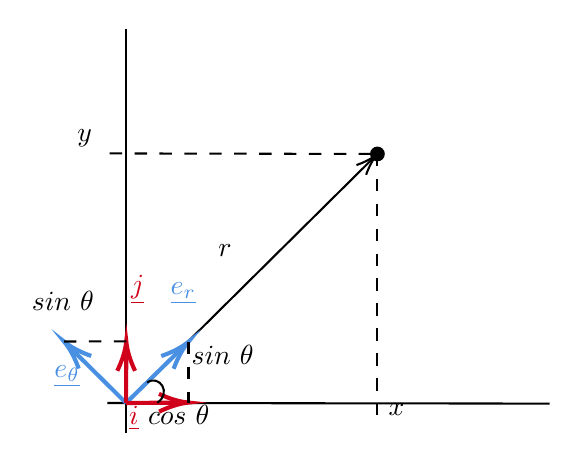
\begin{tikzpicture}[x=0.75pt,y=0.75pt,yscale=-1,xscale=1]
		%uncomment if require: \path (0,402); %set diagram left start at 0, and has height of 402

		%Straight Lines [id:da4134121928340384] 
		\draw    (270.1,119.68) -- (270.1,314.3) ;
		%Straight Lines [id:da5926046353448922] 
		\draw    (261,300) -- (474.1,300.3) ;
		%Straight Lines [id:da5096706615516877] 
		\draw    (270,300) -- (389.68,181.42) ;
		\draw [shift={(391.1,180.02)}, rotate = 135.27] [color={rgb, 255:red, 0; green, 0; blue, 0 }  ][line width=0.75]    (10.93,-3.29) .. controls (6.95,-1.4) and (3.31,-0.3) .. (0,0) .. controls (3.31,0.3) and (6.95,1.4) .. (10.93,3.29)   ;
		%Shape: Circle [id:dp7250045716603137] 
		\draw  [fill={rgb, 255:red, 0; green, 0; blue, 0 }  ,fill opacity=1 ] (388.05,180.02) .. controls (388.05,178.33) and (389.42,176.97) .. (391.1,176.97) .. controls (392.78,176.97) and (394.15,178.33) .. (394.15,180.02) .. controls (394.15,181.7) and (392.78,183.07) .. (391.1,183.07) .. controls (389.42,183.07) and (388.05,181.7) .. (388.05,180.02) -- cycle ;
		%Straight Lines [id:da348222394877604] 
		\draw  [dash pattern={on 4.5pt off 4.5pt}]  (391.1,180.02) -- (391.1,309.67) ;
		%Straight Lines [id:da6321585739703421] 
		\draw  [dash pattern={on 4.5pt off 4.5pt}]  (262.1,179.77) -- (391.1,180.02) ;
		%Straight Lines [id:da38254164085879216] 
		\draw [color={rgb, 255:red, 74; green, 144; blue, 226 }  ,draw opacity=1 ][line width=1.5]    (270,300) -- (297.96,272.6) ;
		\draw [shift={(300.1,270.5)}, rotate = 135.58] [color={rgb, 255:red, 74; green, 144; blue, 226 }  ,draw opacity=1 ][line width=1.5]    (14.21,-4.28) .. controls (9.04,-1.82) and (4.3,-0.39) .. (0,0) .. controls (4.3,0.39) and (9.04,1.82) .. (14.21,4.28)   ;
		%Straight Lines [id:da36292628024938856] 
		\draw [color={rgb, 255:red, 74; green, 144; blue, 226 }  ,draw opacity=1 ][line width=1.5]    (270,300) -- (242.23,272.49) ;
		\draw [shift={(240.1,270.38)}, rotate = 44.73] [color={rgb, 255:red, 74; green, 144; blue, 226 }  ,draw opacity=1 ][line width=1.5]    (14.21,-4.28) .. controls (9.04,-1.82) and (4.3,-0.39) .. (0,0) .. controls (4.3,0.39) and (9.04,1.82) .. (14.21,4.28)   ;
		%Straight Lines [id:da44840860590214315] 
		\draw [color={rgb, 255:red, 208; green, 2; blue, 27 }  ,draw opacity=1 ][line width=1.5]    (270,300) -- (270.09,273.3) ;
		\draw [shift={(270.1,270.3)}, rotate = 90.19] [color={rgb, 255:red, 208; green, 2; blue, 27 }  ,draw opacity=1 ][line width=1.5]    (14.21,-4.28) .. controls (9.04,-1.82) and (4.3,-0.39) .. (0,0) .. controls (4.3,0.39) and (9.04,1.82) .. (14.21,4.28)   ;
		%Straight Lines [id:da7989542731151809] 
		\draw [color={rgb, 255:red, 208; green, 2; blue, 27 }  ,draw opacity=1 ][line width=1.5]    (270,300) -- (297.1,299.82) ;
		\draw [shift={(300.1,299.8)}, rotate = 179.62] [color={rgb, 255:red, 208; green, 2; blue, 27 }  ,draw opacity=1 ][line width=1.5]    (14.21,-4.28) .. controls (9.04,-1.82) and (4.3,-0.39) .. (0,0) .. controls (4.3,0.39) and (9.04,1.82) .. (14.21,4.28)   ;
		%Straight Lines [id:da6303605300239684] 
		\draw  [dash pattern={on 4.5pt off 4.5pt}]  (300.1,270.5) -- (300.1,299.8) ;
		%Straight Lines [id:da1244707927752331] 
		\draw  [dash pattern={on 4.5pt off 4.5pt}]  (240.1,270.38) -- (270.1,270.3) ;
		%Curve Lines [id:da4414328655497084] 
		\draw    (280.1,290.13) .. controls (286.1,286.13) and (292.1,295.13) .. (285.05,299.9) ;

		% Text Node
		\draw (395,299) node [anchor=north west][inner sep=0.75pt]   [align=left] {$\displaystyle x$};
		% Text Node
		\draw (245,167) node [anchor=north west][inner sep=0.75pt]   [align=left] {$\displaystyle y$};
		% Text Node
		\draw (313,222) node [anchor=north west][inner sep=0.75pt]   [align=left] {$\displaystyle r$};
		% Text Node
		\draw (300.1,270.5) node [anchor=north west][inner sep=0.75pt]   [align=left] {$\displaystyle sin\ \theta $};
		% Text Node
		\draw (270,300) node [anchor=north west][inner sep=0.75pt]  [color={rgb, 255:red, 208; green, 2; blue, 27 }  ,opacity=1 ] [align=left] {$\displaystyle \underline{i}$};
		% Text Node
		\draw (271,237) node [anchor=north west][inner sep=0.75pt]  [color={rgb, 255:red, 208; green, 2; blue, 27 }  ,opacity=1 ] [align=left] {$\displaystyle \underline{j}$};
		% Text Node
		\draw (290,240.48) node [anchor=north west][inner sep=0.75pt]  [color={rgb, 255:red, 74; green, 144; blue, 226 }  ,opacity=1 ] [align=left] {$\displaystyle \underline{e_{r}}$};
		% Text Node
		\draw (234,280.48) node [anchor=north west][inner sep=0.75pt]  [color={rgb, 255:red, 74; green, 144; blue, 226 }  ,opacity=1 ] [align=left] {$\displaystyle \underline{e_{\theta }}$};
		% Text Node
		\draw (223.1,244.5) node [anchor=north west][inner sep=0.75pt]   [align=left] {$\displaystyle sin\ \theta $};
		% Text Node
		\draw (279.1,299.5) node [anchor=north west][inner sep=0.75pt]   [align=left] {$\displaystyle cos\ \theta $};


	\end{tikzpicture}
\end{mycenter}

As we can see from the diagram:
$$\underline{e_{r}}= \underline{i}\cos\theta + \underline{j}\sin\theta$$
and
$$\underline{e_{\theta}} = \pm \sin\theta \ \underline{i} + \mp \cos\theta\ \underline{j}$$
because $\underline{e_{r}}$ is {\bf orthogonal} to $\underline{e_{\theta}}$. Use the case from the diagram:
$$\underline{e_{\theta}} = \underline{i}\sin\theta - \underline{j}\cos\theta$$

\begin{definition}[Polar Basis Using Cartesian]
	\begin{flalign*}
		\underline{e_{r}}= \underline{i}\cos\theta + \underline{j}\sin\theta \\
		\underline{e_{\theta}} = \underline{i}\sin\theta - \underline{j}\cos\theta
	\end{flalign*}
\end{definition}

\subsubsection{Properties of Polar Orthonormal Basis}
\begin{theorem}
	Since $\underline{e_r}$ and $\underline{e_\theta}$ are \textbf{orthogonal},
	$$\underline{e_r} \cdot \underline{e_\theta} = 0$$
	(scalar product is 0)
\end{theorem}

\clearpage

\begin{theorem}
	The cross product (\ref{eq:cross-product-formula})
	$$\underline{e_r} \times \underline{e_{\theta}} = 0$$
\end{theorem}
\begin{proof}
	$$\begin{aligned} \underline{e_{r}} \times \underline{e_{\theta}} & = (\underline{i}\cos\theta + \underline{j}\sin\theta) \times ( \underline{i}\sin\theta - \underline{j}\cos\theta) \\ \\ &= (\cos^{2}\theta+ \sin^{2}\theta)\underline{i} \times \underline{j} \\ \\
                                                                & = \underline{k}                                                                                                   \\ \\\end{aligned}$$
\end{proof}

\subsection{Derivatives of Polar Orthonormal Basis Vectors}
We assume that the {\bf angle changes with time}, i.e.
$$\theta = \theta\left( t \right) $$
and therefore the {\bf polar basis vectors} are {\bf NOT CONSTANT}.

\subsubsection{First Derivative}
First we will compute the first derivatives $\underline{\dot{e_{r}}}$ and $\underline{\dot{e_{\theta}}}$.
\begin{enumerate}
	\item Computing $\underline{\dot{e_r}}$
	      $$\begin{aligned} \underline{\dot{e_{r}}} & = \frac{d}{dt}\Big(\underline{i}\cos\theta  + \underline{j}\sin\theta\Big)         \\ \\
                                        & = - \dot{\theta}\sin(\theta) \underline{i} + \dot{\theta}\cos(\theta)\underline{j} \\ \\
                                        & = \dot{\theta}(-\sin(\theta)\underline{i} + \cos(\theta)\underline{j})             \\ \\
                                        & = \dot{\theta}\ \underline{e_{\theta}}\end{aligned}$$
	      \begin{definition}[First derivative of $\underline{e_r}$]
		      $$\begin{aligned} \underline{\dot{e_{r}}} &= \dot{\theta}\ \underline{e_{\theta}}\\ \\ &= - \dot{\theta}\sin(\theta) \underline{i} + \dot{\theta}\cos(\theta)\underline{j} \end{aligned}$$
	      \end{definition}

	      \clearpage
	\item Computing $\underline{\dot{e_{\theta}}}$
	      $$\begin{aligned} \underline{\dot{e_{r}}} & = \frac{d}{dt}\Big(-\sin(\theta)\underline{i}  + \cos(\theta)\underline{j}\Big)    \\ \\
                                        & = - \dot{\theta}\cos(\theta) \underline{i} - \dot{\theta}\sin(\theta)\underline{j} \\ \\
                                        & = -\dot{\theta}(\cos(\theta)\underline{i} + \sin(\theta)\underline{j})             \\ \\
                                        & = \dot{\theta}\ \underline{e_{r}}\end{aligned}$$

	      \begin{definition}[First derivative of $\underline{e_r}$]
		      $$\begin{aligned} \underline{\dot{e_{\theta}}} &= -\dot{\theta}\ \underline{e_{r}}\\ \\ &= - \dot{\theta}\cos(\theta) \underline{i} - \dot{\theta}\sin(\theta)\underline{j} \end{aligned}$$
	      \end{definition}
\end{enumerate}
